\section{Overview of Literature}\label{overview}
This section presents literature containing background information on image processing, both background studies and already existing solutions to similar problems. There has not been any suggestions from existing literature on how to solve this exact problem, but there are many different approaches that solves parts of the problem.
Below follows articles and books providing theory and solutions for removing noise from underwater images.

\subsection{Digital Image Processing (Gonzalez and Woods, 2008)}
This book has been the leading book in its field for a long period of time. It gives a simple introduction to image processing, explaining the fundamentals and giving examples. It does not give complete solutions or complex algorithms, but it helps getting familiar with the basics and to understand how the computer sees images relative to how humans see them.

The book explains simple procedures as a averaging filter and median filter, which can be used to blur or sharpen the image. 

It also explains more complex procedures as morphological operators with eroding and dilating and Fourier filtering. 

Eroding and dilating can be used to sharpen an image, or it can be used to remove particles from the image by reducing the size of objects until the unwanted objects disappear and then again expand the main object until it reaches its original size. 

Fourier filtering shows how to transform the image from the spatial domain into the frequency domain. In the frequency domain it is possible to remove some frequencies, and then transform the image back to the spatial domain. This can be used to remove light scattering from an image, which can be useful to remove in some underwater images.

\subsection{Machine Vision (Jain, Kasturi and Schunck, 1995)}

\subsection{Underwater Image Processing: State of the Art of \\
Restoration and Image Enhancement Methods \\
(Raimondo Schettini and Silvia Corchs, 2010)}
The paper by Raimondo Schettini and Silvia Corchs explains the problems with underwater image processing due to the light propagation in the water medium. The physical properties of water cause degradation effects not present in images taken in air. The water absorbs light and therefore limits the visibility distance, and it also causes scattering, which changes the direction of the light path. This influences the overall performance of underwater imaging systems. Forward scattering is the spreading of light from an object towards the camera, while backward scattering is the light reflected by the water towards the camera before it actually reaches an object. Backward scattering reduces the contrast of the image, and is seen as sunbeams on the image. Scattering comes from not only the water, but all particles in the water. 

\begin{figure}[h]
    \centering
    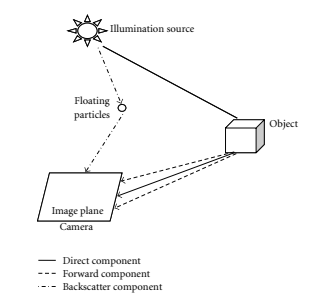
\includegraphics[width=0.7\textwidth]{Images/image_from_paper}
    \caption{Explanation of scattering from (Raimondo Schettini and Silvia Corchs, 2010, p. 3)}
    \label{fig:image_from_paper}
\end{figure}

The paper explains different sub-problems and what approaches that can be used to solve them. There are many example images with clear improvement, but the paper does not contain any examples on implementation. Some of the techniques mentioned in the paper are MTF, ACE, Bazeille et al, Iqbal et al and Petit et al. The paper also contains a table of all relevant techniques, with a brief description and usage area.

{\color{red}Try out some of these techniques???}


\subsection{OpenCV Online Tutorial \\
(http://docs.opencv.org/2.4/doc/tutorials/tutorials.html)}
To learn about the OpenCV library and its functionality this online tutorial was quite useful. It contains many good examples on different implementations and how to use the functions in the OpenCV library. All functionality is explained very well with goal, theory on the topic, code, explanation of the code and results. These tutorials made it very easy getting started with OpenCV.
